\usetikzlibrary{arrows.meta,patterns,shapes.misc}

\begin{frame}{priority queue}
    \begin{itemize}
    \item assign priorities to flows
    \item drop packet from lowest priority flow possible
    \item on ties, choose other drop strategy
    \end{itemize}
\end{frame}

\begin{frame}{priority-based dequeue}
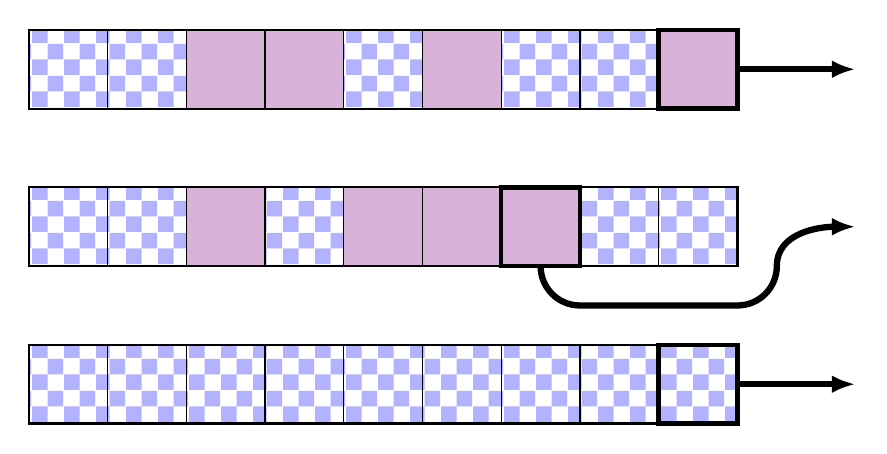
\begin{tikzpicture}
\tikzset{
    first flow/.style={pattern=checkerboard,pattern color=blue!30},
    second flow/.style={fill=violet!30},
    ghost/.style={dashed,fill opacity=0.5},
    packet move line/.style={draw,line width=0.8mm},
}
    \begin{scope}[yshift=0cm]
        \foreach \x in {0,1,4,6,7} {
            \path[first flow] (\x, -.5) rectangle ++(1, 1);
        }
        \foreach \x in {2,3,5,8} {
            \path[second flow] (\x, -.5) rectangle ++(1, 1);
        }
        \draw[thick] (0, -.5) rectangle (9, .5);
        \foreach \x in {0,1,2,3,4,5,6,7,8} {
            \draw (\x, -.5) -- (\x, .5);
        }
        \draw[ultra thick] (8, -.5) rectangle ++(1,1);
        \path[packet move line,-{Latex[length=3mm]}] (9, 0) -- ++(1.5, 0);
    \end{scope}

    \begin{scope}[yshift=-2cm]
        \foreach \x in {0,1,3,7,8} {
            \path[first flow] (\x, -.5) rectangle ++(1, 1);
        }
        \foreach \x in {2,4,5,6} {
            \path[second flow] (\x, -.5) rectangle ++(1, 1);
        }
        \draw[thick] (0, -.5) rectangle (9, .5);
        \foreach \x in {0,1,2,3,4,5,6,7,8} {
            \draw (\x, -.5) -- (\x, .5);
        }
        \draw[ultra thick] (6, -.5) rectangle ++(1,1);
        \path[packet move line,-{Latex[length=3mm]}] (6.5, -.5) to[out=-90,in=180] ++(.5, -.5)
            -- ++(2, 0) to[out=0,in=-90] ++(.5, .5) to[in=180,out=90] ++(1, .5);
    \end{scope}
    
    \begin{scope}[yshift=-4cm]
        \foreach \x in {0,1,2,3,4,5,6,7,8} {
            \path[first flow] (\x, -.5) rectangle ++(1, 1);
        }
        \foreach \x in {} {
            \path[second flow] (\x, -.5) rectangle ++(1, 1);
        }
        \draw[thick] (0, -.5) rectangle (9, .5);
        \foreach \x in {0,1,2,3,4,5,6,7,8} {
            \draw (\x, -.5) -- (\x, .5);
        }
        \draw[ultra thick] (8, -.5) rectangle ++(1,1);
        \path[packet move line,-{Latex[length=3mm]}] (9, 0) -- ++(1.5, 0);
    \end{scope}
\end{tikzpicture}
\end{frame}

\begin{frame}{priority-based dropping}
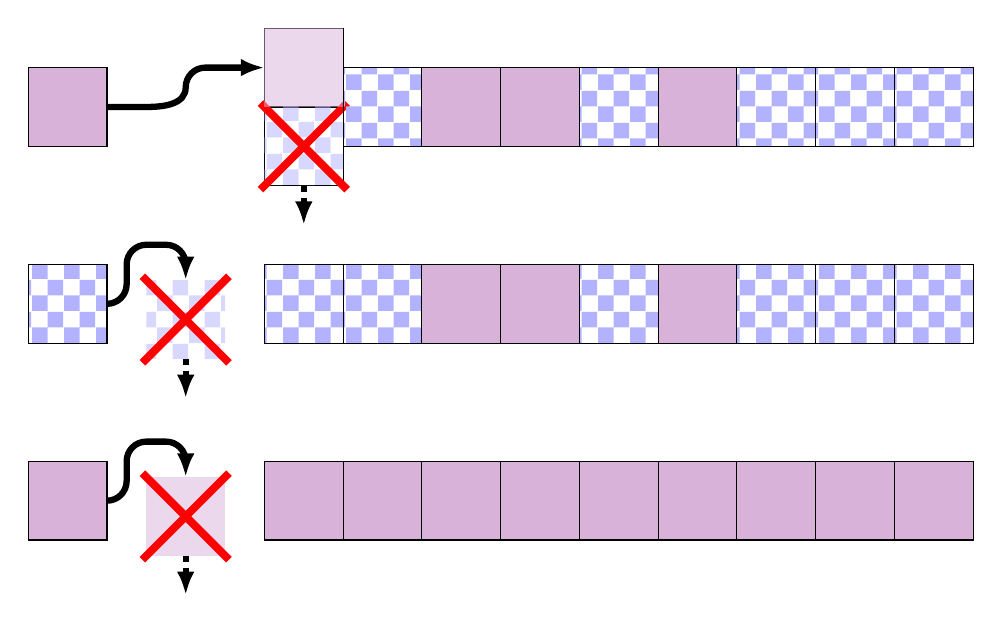
\begin{tikzpicture}
\tikzset{
    first flow/.style={pattern=checkerboard,pattern color=blue!30},
    second flow/.style={fill=violet!30},
    ghost/.style={dashed,fill opacity=0.5},
    packet move line/.style={draw,line width=0.8mm},
}
    \begin{scope}[yshift=-2cm]
        \foreach \x in {0} {
            \draw (\x, -1) rectangle ++(1,1);
            \draw (\x, 0) rectangle ++(1,1);
            \path[first flow,ghost] (\x, -1) rectangle ++(1, 1);
            \node[cross out,draw=red,line width=1mm,minimum width=1cm,minimum height=1cm] at (\x+.5, -.5) {};
            \path[second flow,ghost] (\x, 0) rectangle ++(1, 1);
        }
        \foreach \x in {1,4,6,7,8} {
            \path[first flow] (\x, -.5) rectangle ++(1, 1);
        }
        \foreach \x in {-3,2,3,5} {
            \path[second flow] (\x, -.5) rectangle ++(1, 1);
        }
        \foreach \x in {1,2,3,4,5,6,7,8} {
            \draw (\x, -.5) -- (\x, .5);
        }
        \path[draw] (1, -.5) rectangle (9, .5);
        \path[draw] (-3, -.5) rectangle (-2, .5);
        \path[packet move line,-{Latex[length=3mm]}] (-2, 0) -- (-1.5, 0) to[in=270,out=0]
            (-1., .25) to[in=180,out=90] (-0.75, .5) -- (0, .5);
        \path[packet move line,dotted,-{Latex[length=3mm]}] (.5,-1) -- ++(0, -.5cm);% node[below=-2mm] {discarded};
    \end{scope}
    \begin{scope}[yshift=-4.5cm]
        \foreach \x in {-1.5} {
            \path[first flow,ghost] (\x, -.7) rectangle ++(1, 1);
            \node[cross out,draw=red,line width=1mm,minimum width=1cm,minimum height=1cm] at (\x+.5, -.2) {};
        }
        \foreach \x in {-3,0,1,4,6,7,8} {
            \path[first flow] (\x, -.5) rectangle ++(1, 1);
        }
        \foreach \x in {2,3,5} {
            \path[second flow] (\x, -.5) rectangle ++(1, 1);
        }
        \foreach \x in {1,2,3,4,5,6,7,8} {
            \draw (\x, -.5) -- (\x, .5);
        }
        \path[draw] (0, -.5) rectangle (9, .5);
        \path[draw] (-3, -.5) rectangle (-2, .5);
        \path[packet move line,-{Latex[length=3mm]}] (-2, 0) -- (-2.0, 0) to[in=270,out=0] (-1.75, 0.25) -- (-1.75, .5) to[in=180,out=90] (-1.5, 0.75)
           -- (-1.25, 0.75) to[out=0,in=45+90-45] (-1, .5) -- (-1, -.2+.5);
        \path[packet move line,dotted,-{Latex[length=3mm]}] (-1,-.7) -- ++(0, -.5cm);% node[below=-2mm] {discarded};
    \end{scope}
    \begin{scope}[yshift=-7cm]
        \foreach \x in {-1.5} {
            \path[second flow,ghost] (\x, -.7) rectangle ++(1, 1);
            \node[cross out,draw=red,line width=1mm,minimum width=1cm,minimum height=1cm] at (\x+.5, -.2) {};
        }
        \foreach \x in {-3,0,1,2,3,4,5,6,7,8} {
            \path[second flow] (\x, -.5) rectangle ++(1, 1);
        }
        \foreach \x in {1,2,3,4,5,6,7,8} {
            \draw (\x, -.5) -- (\x, .5);
        }
        \path[draw] (0, -.5) rectangle (9, .5);
        \path[draw] (-3, -.5) rectangle (-2, .5);
        \path[packet move line,-{Latex[length=3mm]}] (-2, 0) -- (-2.0, 0) to[in=270,out=0] (-1.75, 0.25) -- (-1.75, .5) to[in=180,out=90] (-1.5, 0.75)
           -- (-1.25, 0.75) to[out=0,in=45+90-45] (-1, .5) -- (-1, -.2+.5);
        \path[packet move line,dotted,-{Latex[length=3mm]}] (-1,-.7) -- ++(0, -.5cm);% node[below=-2mm] {discarded};
    \end{scope}
\end{tikzpicture}
\end{frame}

\begin{frame}{priority-based dropping (alt)}
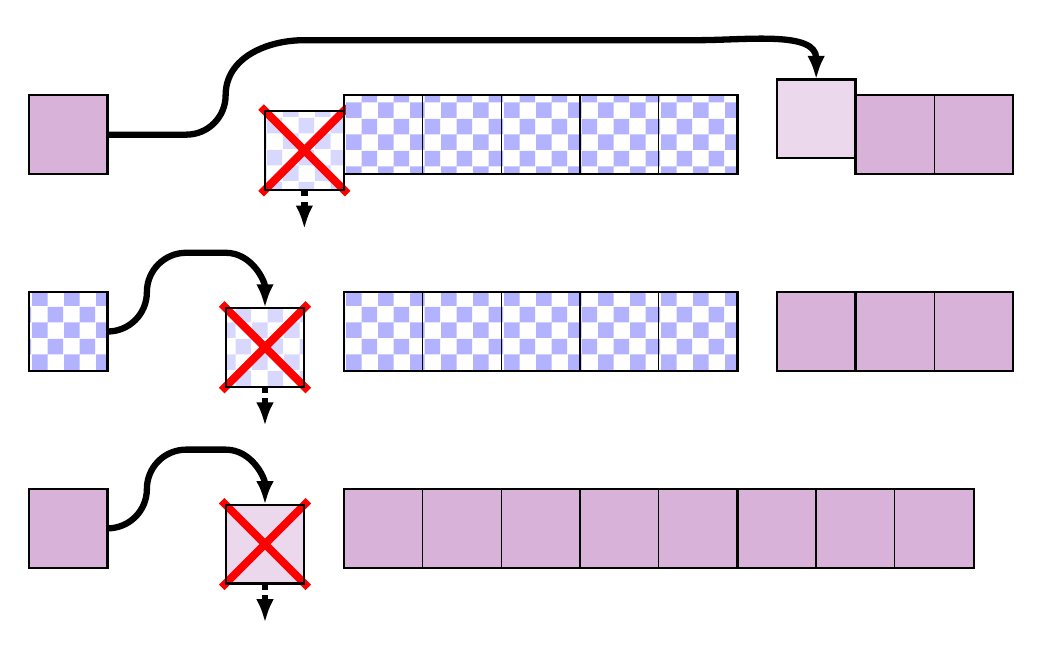
\begin{tikzpicture}
\tikzset{
    first flow/.style={pattern=checkerboard,pattern color=blue!30},
    second flow/.style={fill=violet!30},
    ghost/.style={dashed,fill opacity=0.5},
    packet move line/.style={draw,line width=0.8mm},
}
    \begin{scope}[yshift=-2cm]
        \foreach \x in {-1} {
            \path[first flow,ghost] (\x, -.7) rectangle ++(1, 1);
            \node[cross out,draw=red,line width=1mm,minimum width=1cm,minimum height=1cm] at (\x+.5, -.2) {};
        }
        \foreach \x in {0,1,2,3,4} {
            \path[first flow] (\x, -.5) rectangle ++(1, 1);
        }
        \foreach \x in {5.5} {
            \path[second flow,ghost] (\x, -.3) rectangle ++(1, 1);
        }
        \foreach \x in {-4,6.5,7.5} {
            \path[second flow] (\x, -.5) rectangle ++(1, 1);
        }
        \path[draw,thick] (-4, -.5) rectangle (-3, .5);
        \draw[thick] (0, -.5) rectangle (5, .5);
        \draw[thick] (5.5, -.3) rectangle ++(1, 1);
        \draw[thick] (-1, -.7) rectangle ++(1, 1);
        \draw[thick] (6.5, -.5) rectangle (8.5, .5);
        \foreach \x in {0,1,2,3,4,6.5,7.5,8.5} {
            \draw (\x, -.5) -- (\x, .5);
        }
        \path[packet move line,-{Latex[length=3mm]}] (-3, 0) -- (-2.0, 0) to[in=270,out=0] (-1.5, 0.5) to[in=180,out=90] (-.5, 1.2)
           -- (4.5, 1.2) to[out=0,in=45+90-45] (6, 0.7);
        \path[packet move line,dotted,-{Latex[length=3mm]}] (-.5,-.7) -- ++(0, -.5cm);% node[below=-2mm] {discarded};
    \end{scope}
    \begin{scope}[yshift=-4.5cm]
        \foreach \x in {-1.5} {
            \path[first flow,ghost] (\x, -.7) rectangle ++(1, 1);
            \node[cross out,draw=red,line width=1mm,minimum width=1cm,minimum height=1cm] at (\x+.5, -.2) {};
        }
        \foreach \x in {-4,0,1,2,3,4} {
            \path[first flow] (\x, -.5) rectangle ++(1, 1);
        }
        \foreach \x in {5.5,6.5,7.5} {
            \path[second flow] (\x, -.5) rectangle ++(1, 1);
        }
        \path[draw,thick] (-4, -.5) rectangle (-3, .5);
        \draw[thick] (0, -.5) rectangle (5, .5);
        \draw[thick] (5.5, -.5) rectangle ++(1, 1);
        \draw[thick] (-1.5, -.7) rectangle ++(1, 1);
        \draw[thick] (6.5, -.5) rectangle (8.5, .5);
        \foreach \x in {0,1,2,3,4,6.5,7.5,8.5} {
            \draw (\x, -.5) -- (\x, .5);
        }
        \path[packet move line,-{Latex[length=3mm]}] (-3, 0) -- (-3.0, 0) to[in=270,out=0] (-2.5, 0.5) to[in=180,out=90] (-2, 1)
           -- (-1.5, 1) to[out=0,in=45+90-45] (-1, -.2+.5);
        \path[packet move line,dotted,-{Latex[length=3mm]}] (-1,-.7) -- ++(0, -.5cm);% node[below=-2mm] {discarded};
    \end{scope}
    \begin{scope}[yshift=-7cm]
        \foreach \x in {-1.5} {
            \path[second flow,ghost] (\x, -.7) rectangle ++(1, 1);
            \node[cross out,draw=red,line width=1mm,minimum width=1cm,minimum height=1cm] at (\x+.5, -.2) {};
        }
        \foreach \x in {-4,0,1,2,3,4} {
            \path[second flow] (\x, -.5) rectangle ++(1, 1);
        }
        \foreach \x in {5,6,7} {
            \path[second flow] (\x, -.5) rectangle ++(1, 1);
        }
        \path[draw,thick] (-4, -.5) rectangle (-3, .5);
        \draw[thick] (0, -.5) rectangle (5, .5);
        \draw[thick] (5, -.5) rectangle ++(1, 1);
        \draw[thick] (-1.5, -.7) rectangle ++(1, 1);
        \draw[thick] (6, -.5) rectangle (8, .5);
        \foreach \x in {0,1,2,3,4,6,7,8} {
            \draw (\x, -.5) -- (\x, .5);
        }
        \path[packet move line,-{Latex[length=3mm]}] (-3, 0) -- (-3.0, 0) to[in=270,out=0] (-2.5, 0.5) to[in=180,out=90] (-2, 1)
           -- (-1.5, 1) to[out=0,in=45+90-45] (-1, -.2+.5);
        \path[packet move line,dotted,-{Latex[length=3mm]}] (-1,-.7) -- ++(0, -.5cm); % node[below=-2mm] {discarded};
    \end{scope}
\end{tikzpicture}
\end{frame}

\begin{frame}{priority: all or nothing}
    \begin{itemize}
    \item if flow A has greater priority than flow B
    \item and both can use full available bandwidth
    \vspace{.5cm}
    \item flow A gets full available bandwidth
    \item flow B gets no bandwidth (everything dropped)
    \end{itemize}
\end{frame}

